\section{Spectra Access}
\label{sec:spectra_access}

%%%%%%%---- BEGIN ----  ----%%%%%%
\begin{frame}
  \frametitle{Spectra Access}

  \begin{columns}[T]

      \begin{column}{.3\textwidth}
        \centering
        \vspace{0.5em}
\includegraphics[width=.8\textwidth]{gfx/logo_relab}\\
        \vspace{0.5em}
\includegraphics[width=.6\textwidth]{gfx/logo_sshade}\\
        \vspace{0.5em}
\includegraphics[width=.8\textwidth]{gfx/logo_m4ast}\\
        \vspace{0.5em}
\includegraphics[width=.8\textwidth]{gfx/logo_classy}\\
      \end{column}


    \begin{column}{.7\textwidth}
      \begin{overlayarea}{\textwidth}{\textheight}
        \vspace{1em}

        \begin{itemize}[<.->]
          \item \emph{\bf Spectra are complex data products}
            \begin{itemize}[<.->]
              \item[$\circ$] Wavelength, Reflectance, Irradiance, \dots
              \item[$\circ$] Instrument Metadata
              \item[$\circ$] Sample Metadata
            \end{itemize}
        \vspace{1em}
          \item \emph{\bf Spectra Databases for Ast./Comets/Met.}
            \begin{itemize}[<.->]
              \item[$\circ$] PDS, CDS, RELAB
              \item[$\circ$] SMASS, MITHNEOS
            \end{itemize}
        \vspace{1em}
          \item \emph{\bf Spectra Aggregators for Asteroids and Meteorites}
            \begin{itemize}[<.->]
              \item[$\circ$] SSHADE, M4AST, classy
              \item[$\circ$] Processing required
              \item[$\circ$] Few updates
            \end{itemize}

        \end{itemize}
      \end{overlayarea}
    \end{column}

  \end{columns}

\end{frame}

\begin{frame}[t]{Demo}
  The next slides show an outline of the demoed material.
\end{frame}

\begin{frame}[t]{M4AST}
  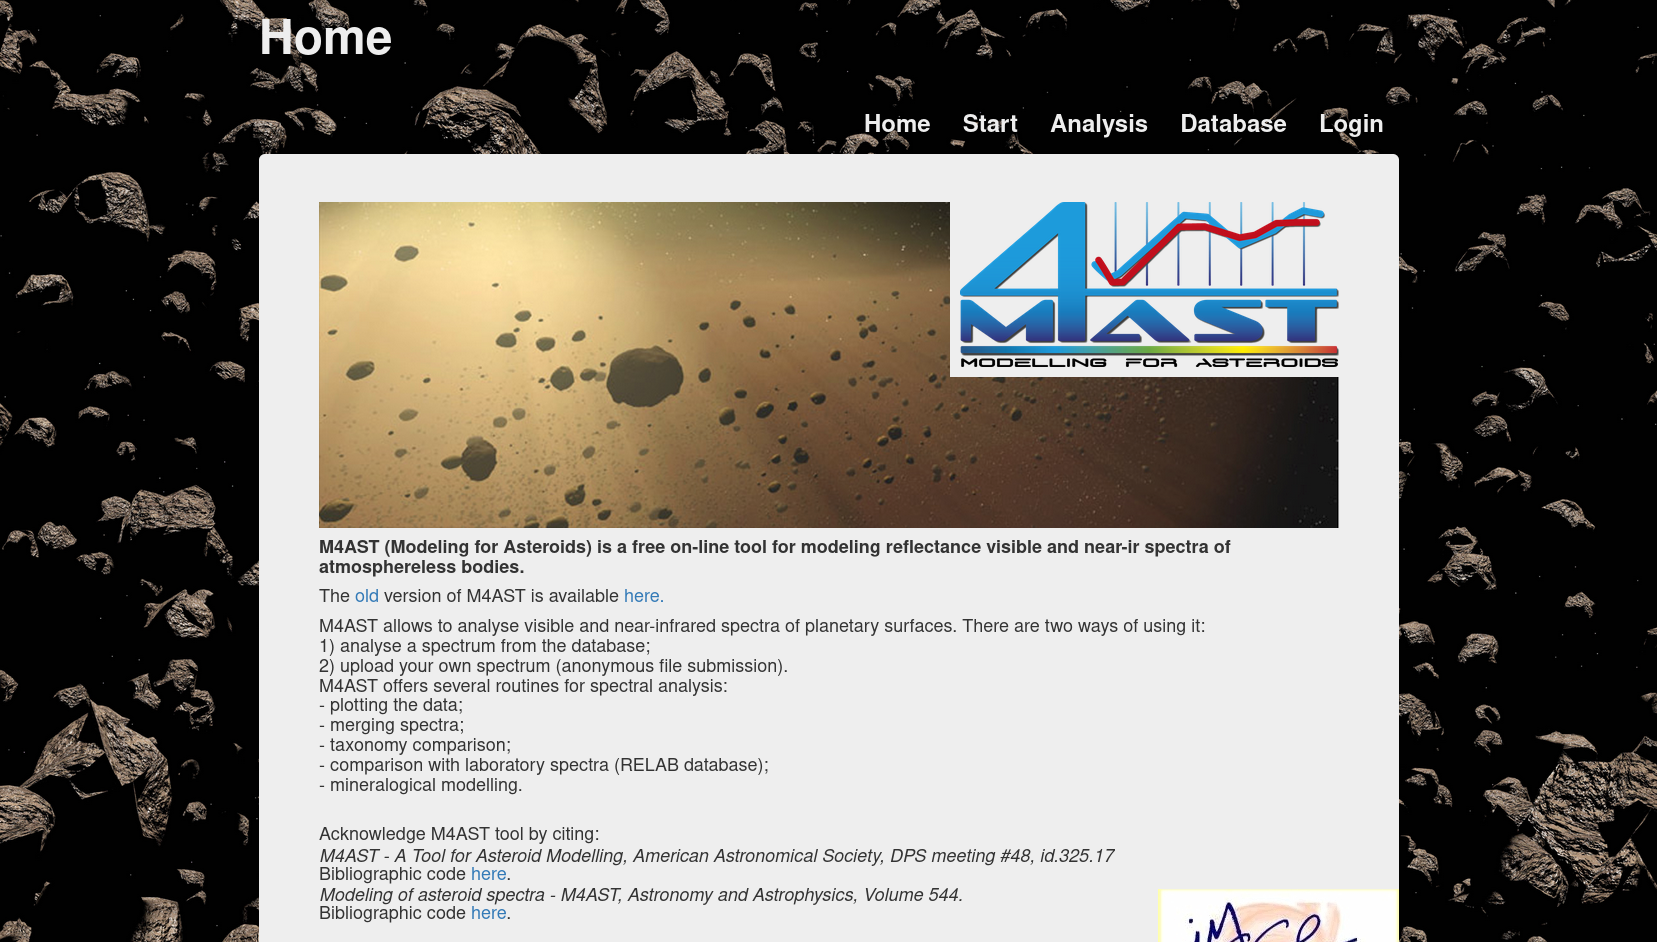
\includegraphics[width=0.8\textwidth]{gfx/demo_m4ast}
  \url{https://spectre.imcce.fr/m4ast/index.php/index/home}
\end{frame}

\begin{frame}[t]{classy}
  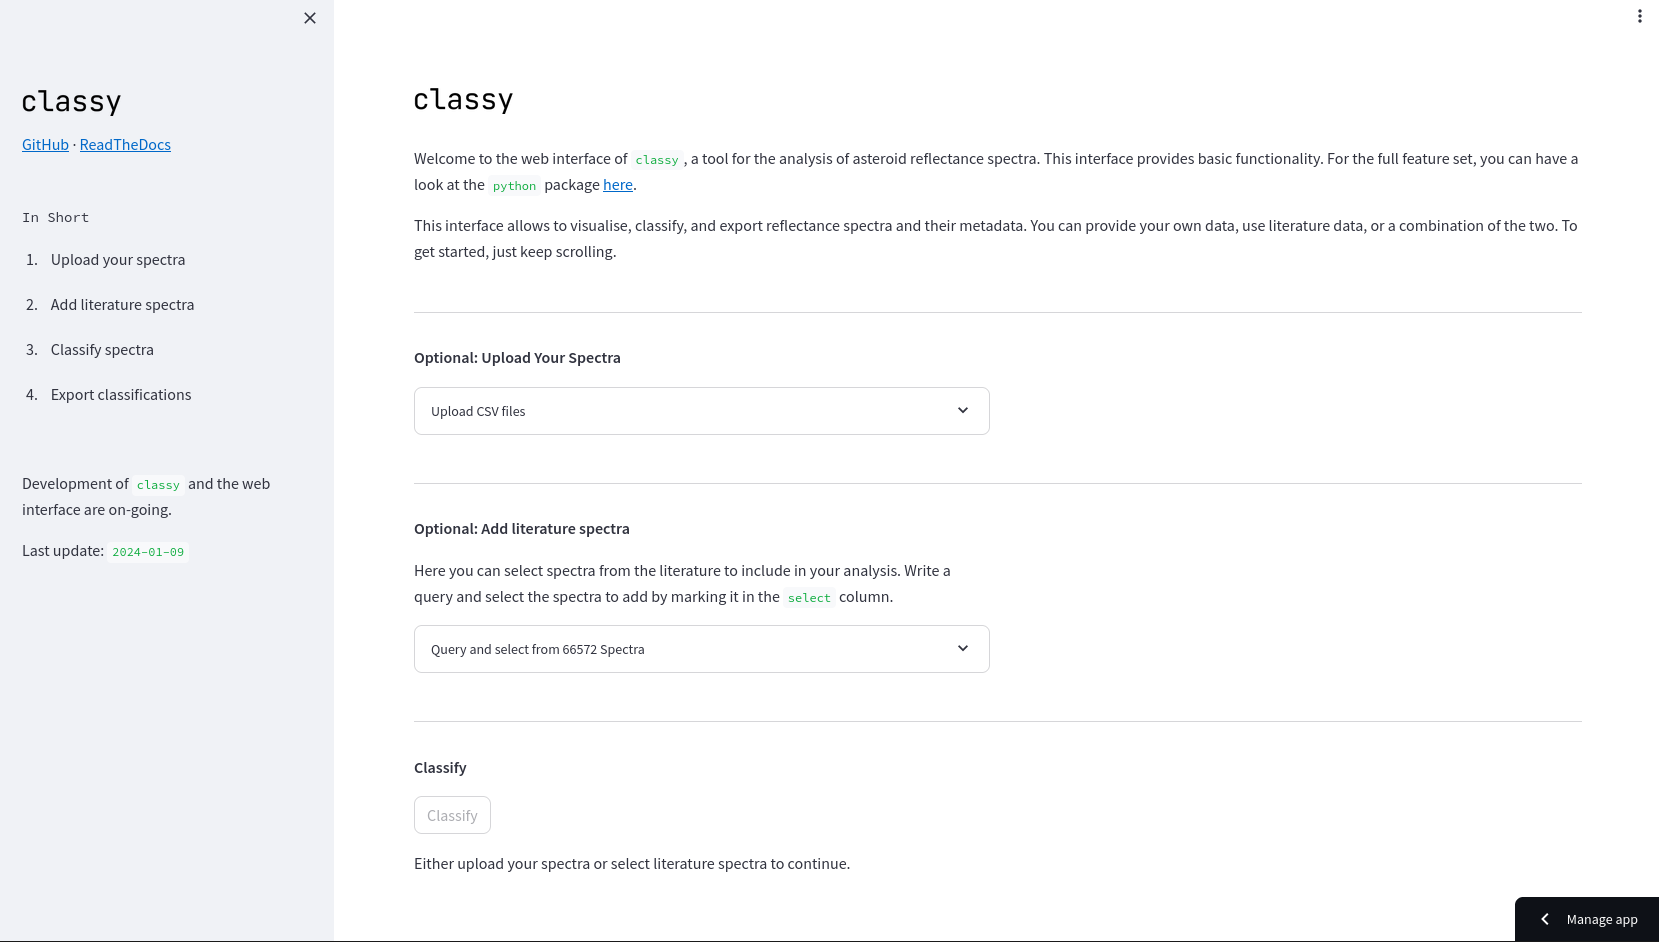
\includegraphics[width=0.8\textwidth]{gfx/demo_classy}
  \url{https://classy.streamlit.app/}
\end{frame}

\begin{frame}[t]{RELAB}
  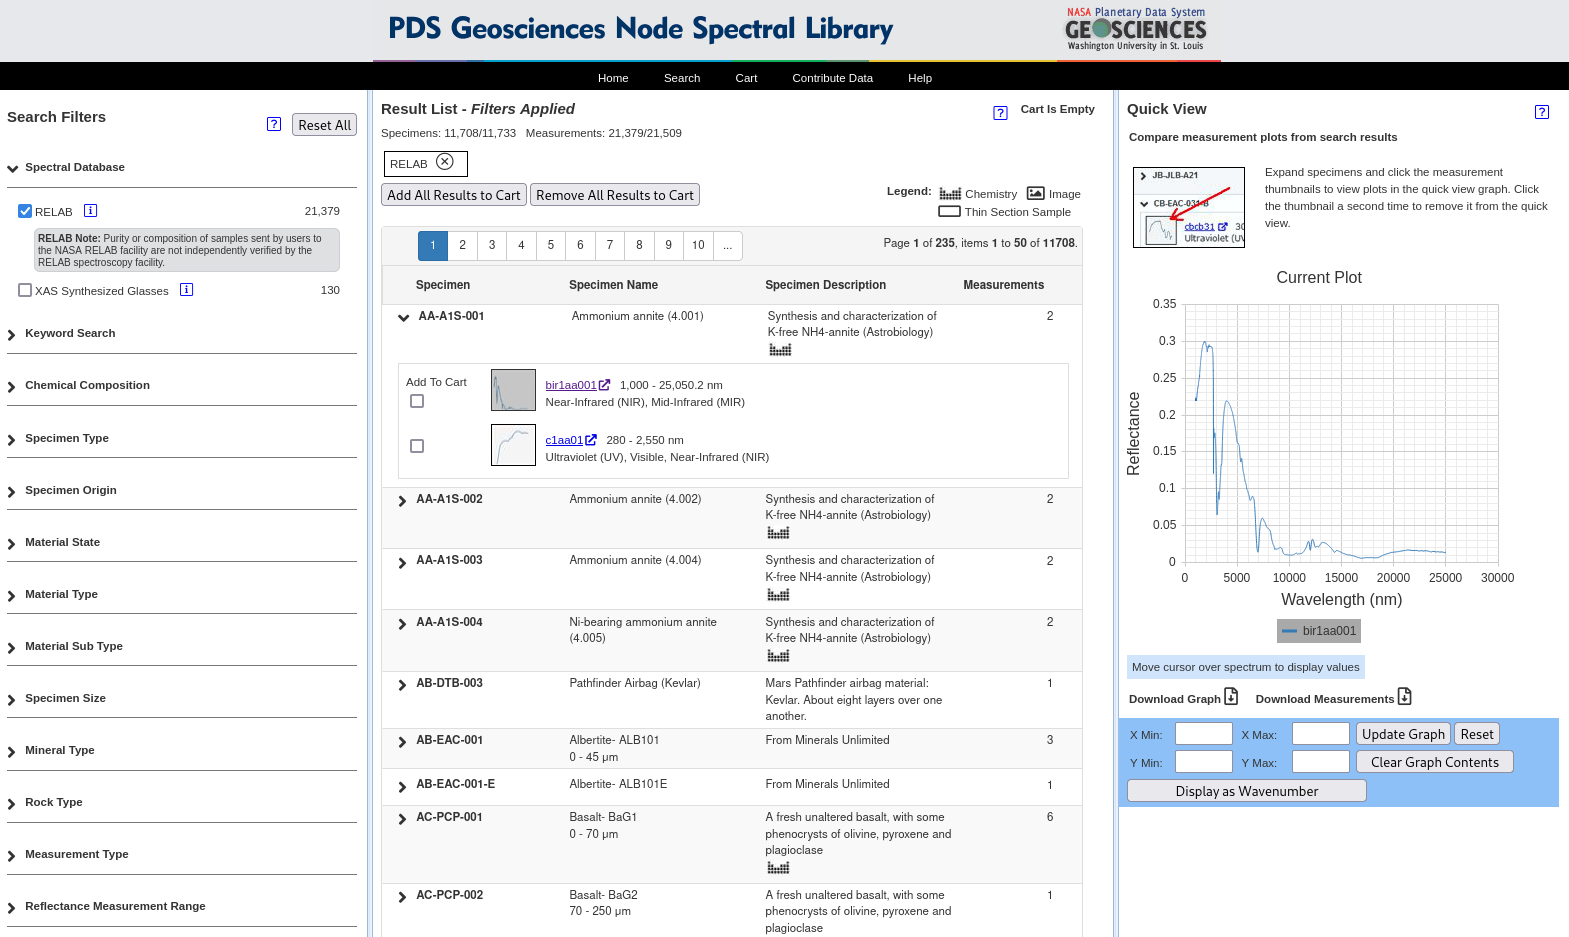
\includegraphics[width=0.8\textwidth]{gfx/demo_relab}
  \url{https://sites.brown.edu/relab/relab-spectral-database/}
\end{frame}

\begin{frame}[t]{SSHADE}
  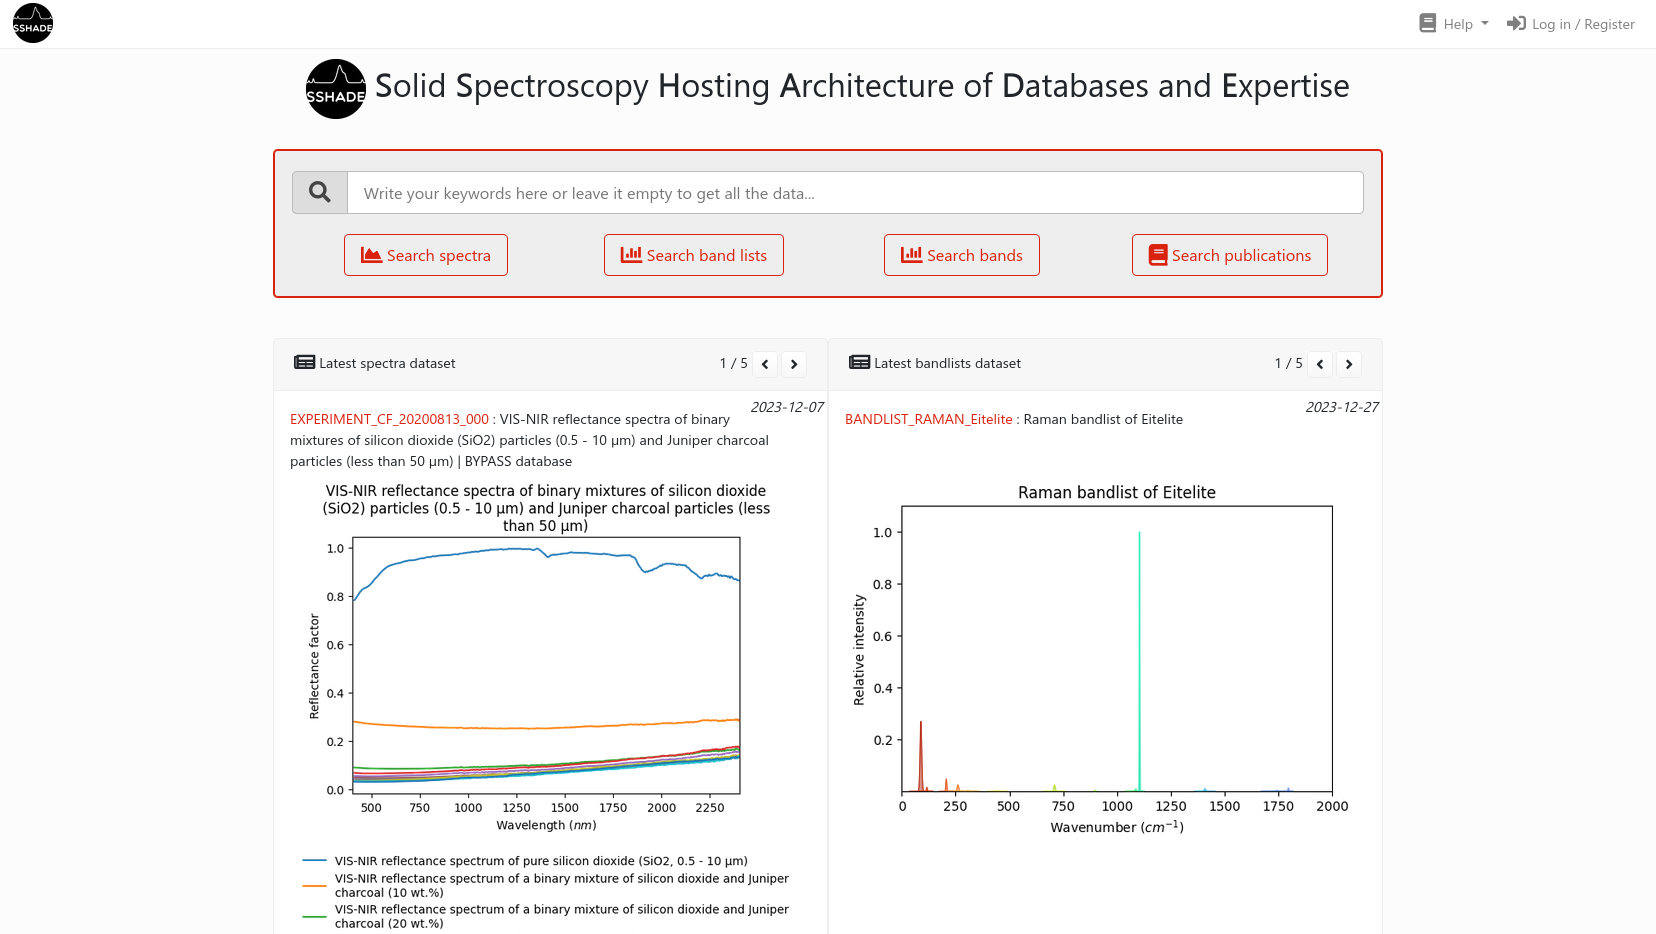
\includegraphics[width=0.8\textwidth]{gfx/demo_sshade}
  \url{https://www.sshade.eu}
\end{frame}

\begin{frame}[t]{SSHADE}
  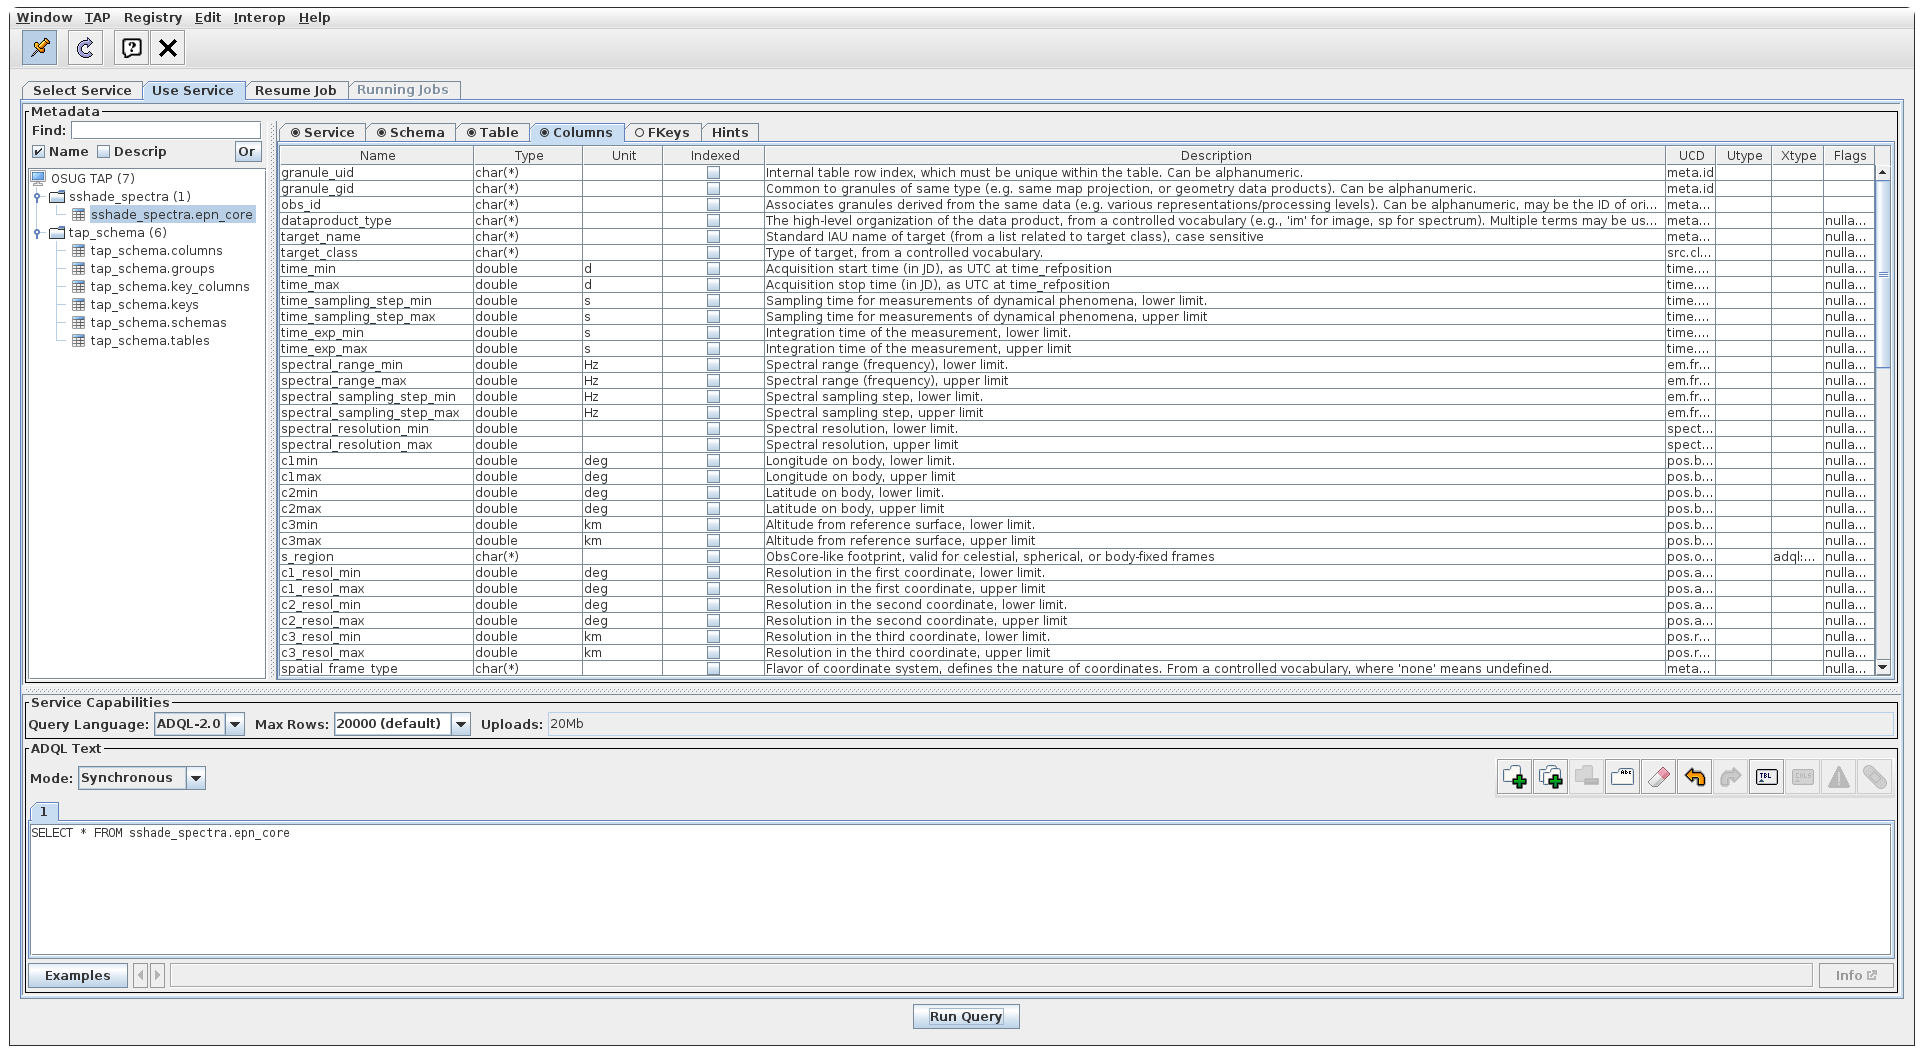
\includegraphics[width=0.8\textwidth]{gfx/demo_tap}\\
  % + missing TAP documentation\\
  % + TAP discovery in TOPCAT
  TOPCAT \textrightarrow~TAP Query \textrightarrow~``SSHADE''
\end{frame}

\begin{frame}[t]{Tutorial}
  [20min] Tutorial notebook on spectra access with SSHADE and TAP
  % Code for classy but without running it [?]
\end{frame}
